\chapter{Particle transport and lagrangian drifts}
\label{ch:part:transp}

\section{Drogues displacements}
\label{sec:drog:displ}
During a hydrodynamic simulation, \telemac{2D} offers the possibility
of monitoring the tracks followed by some particles (drogues) introduced
into the fluid from outflow points.
The result is produced in the form of a Tecplot format file or a binary PCL
format file containing the various positions of the drogues in time,
see paragraph \ref{subs:drog:output:file} for more details.

Note that using this feature provides more accurate results than using
the particle tracking features of the post-processing tools.
Contrary to \telemac{2D} for which monitoring floats is determined at each time
step, the post-processing tools are based on the \telkey{RESULTS FILE}
that is usually sampled much coarser.
Since release 7.0, the management of drogues is modified to be coherent with
other particle transport features of \telemac{2D} (oil spill and algae).
Hereafter, we give the implementation details.

\subsection{Input Files}
\label{subs:drog:inp:fil}
In addition to the mandatory files for a classical \telemac{2D} model
(steering, geometry, boundary conditions),
there is the option to use an input file containing a number of polygons
that specify an initial particle distribution.

\subsection{Steering file}
\label{subs:drog:steer:file}
The following steering file keywords relate to drogues.
The same keywords are used for oil spill and algae.

\begin{itemize}
\item The maximum number of allowed particles:
\telkey{MAXIMUM NUMBER OF DROGUES}.
This is the number used to allocate various arrays.

\item The drogues printout period: \telkey{PRINTOUT PERIOD FOR DROGUES}.
This sets the time step interval between successive outputs to the
drogues output file,

\item The name of the output file containing the drogues positions:
\telkey{ASCII DROGUES FILE} (Tecplot format)
or \telkey{BINARY DROGUES FILE} (binary PCL format).
In the case of the PCL format, the file extension should be “.pcl”
(See section \ref{subs:drog:output:file}),

\item \telkey{DROGUES FILE FORMAT}: TECPLOT or BKBINPCL.
If TECPLOT is chosen, the \telkey{ASCII DROGUES FILE} is written.
If BKBINPCL is chosen, the \telkey{BINARY DROGUES FILE} is written,

\item The file which specifies initial drogues placement
and the class of each particle:
\telkey{DROGUES INITIAL POSITIONING DATA FILE}.
The $z$ coordinate sets the class of each particle,

\item The format of the file that specifies initial drogues displacement:
\telkey{FORMAT OF THE DROGUES POSITIONING DATA FILE}.
Currently, the only option is BKASCI2S (BlueKenue i2s),

\item The number of drogues per unit area for each drogue class
(one number for each class): \telkey{INITIAL DROGUES SAMPLING DENSITY},

\item \telemac{2D} offers the possibility to introduce a stochastic diffusion
coefficient.
When setting the keyword \telkey{STOCHASTIC DIFFUSION MODEL} = 1 (default = 0),
a stochastic model will generate stochastically a diffusion coefficient
which is computed using the turbulent viscosity.
If no turbulence is activated, this stochastic diffusion is not considered
during the particle transport.
\end{itemize}

\subsection{Initial drogues locations}
\label{subs:drog:init}
The initial drogues locations can be specified in three ways.
Any combination of these three ways can be used.

\begin{enumerate}
\item The geometry file.
An extra variable can be included in the geometry file, called DROGUES CLASSES.
An extra variable can be added to the \telkey{GEOMETRY FILE} using BlueKenue.
This variable specifies the drogues class.
The number of drogues per unit area for each class is specified by the keyword
\telkey{INITIAL DROGUES SAMPLING DENSITY}.
\telkey{\subparagraph*{Detailed BlueKenue steps:}
\begin{itemize}
\item Load existing geometry file (File, Open...),
\item Create new Selafin file (File, New > SELAFIN Object...),
\item Drag bathymetry variable from existing geometry to new Selafin object.
\item Select the bathymetry variable, then start the Calculator (Tools, Calculator...),
\item Select the bathymetry variable as A,
\item Type a*0 in the Expression box (this defines a variable everywhere equal to 0),
\item Give the Result Name as DROGUES CLASSES,
\item Create a Polygon (see item 2) covering the area of the drogues,
with the value equal to the class number,
\item Select the DROGUES CLASSES variable, then select Tools, Map Object...
\item Select the Polygon in Available Objects, then select Yes,
\item Drag DROGUES CLASSES into the new Selafin object,
\item Save the new Selafin object (File, Save).
\end{itemize}	}

\item A polygon file.
The polygon file name is given by the keyword
\telkey{DROGUES INITIAL POSITIONING DATA FILE}.
Each polygon defines an area and a drogues class.
The polygon file can be created using BlueKenue.
The $z$ coordinate sets the class of each particle.
The number of drogues per unit area for each class is specified by the keyword
\telkey{INITIAL DROGUES SAMPLING DENSITY}.
\telkey{\subparagraph*{Detailed BlueKenue steps:}
\begin{itemize}
\item Select New, Closed Line...
\item Use the mouse to click on the position of each polygon point,
\item Select New, Closed Line... again,
\item Type the name of the polygon in the Name box,
\item Type the class value in the Value box,
\item Click OK,
\item Save the polygon in i2s format (File, Save),
\end{itemize}	}

\item The FORTRAN user subroutine \telfile{USER\_FLOT}.
Commented out examples are included in \telfile{USER\_FLOT}.
Within \telfile{USER\_FLOT}, the subroutine \telfile{ADD\_PARTICLE}
can be called.
Each call of \telfile{ADD\_PARTICLE} will add a drogue with a specified
$x$, $y$, tag and class.
Each particle should be defined with a unique tag number.
\end{enumerate}

\subsection{Output file}
\label{subs:drog:output:file}
Besides the classic result file, \telemac{2D} produces a specific output file
for drogues.
This file is a formatted file created by \telemac{2D} during the computation and
can be of two different formats:

\begin{itemize}
\item  a file in the Tecplot format, it is given by the keyword
\telkey{ASCII DROGUES FILE}.
To visualize the drogues positions with Tecplot software, the user must:

\begin{itemize}
\item Use the File$>$Load Data File(s) command to load the \telkey{RESULTS FILE},

\item Use the File$>$Load Data File(s) command to load the Tecplot drogues file.
\end{itemize}

\begin{WarningBlock}{Warning:}
In order to add the Tecplot DROGUES FILE to Telemac result data that was already
loaded, select ``Add to current data'' set in the
\textbf{Load Data File Warning dialogue} (cf. Figure \ref{fig:load:df}).
The Load Data File Warning dialogue will appear after you have selected the file
and zones and/or variables to load.
\end{WarningBlock}
\begin{figure}[!htbp]
\centering
 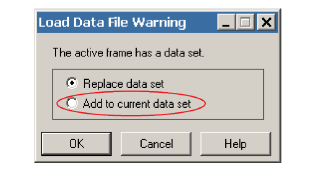
\includegraphics[width=2.77in, height=1.70in, keepaspectratio=false]{./graphics/warning1.png}
 \caption{Warning dialogue box}%
 \label{fig:load:df}
\end{figure}
\item a file in the BlueKenue PCL format, the output file can be read
in to BlueKenue.
The file extension of the file should be “pcl”.
\end{itemize}

\begin{WarningBlock}{Additional drogues output formats:}
\begin{itemize}
\item It is possible to develop additional drogues output formats.
This must be done in the subroutine \telfile{UTIMP\_DROGUES}.
A FORTRAN file including the subroutine \telfile{UTIMP\_DROGUES} with the new
format definition needs to be added with the input files.
The user can choose whether to write to the \telkey{ASCII DROGUES FILE}
or the \telkey{BINARY DROGUES FILE}.
\item It is also possible to convert the \telkey{ASCII DROGUES FILE} in Tecplot
  format to a compatible paraview format.
  This process can be found in notebook documentation
  (``\$HOMETEL/notebooks/pretel/converter.ipynb'')
\end{itemize}
\end{WarningBlock}

\section{Algae modelling}
\label{sec:algae:bloom}
Since release 6.3, \telemac{2D} offers the possibility to simulate algae
transport.
Theoretical aspects about algae physics and modelling can be found
in Joly \cite{Joly2011}.


\subsection{Input files}

Input files for algae modelling are the same as for drogues.


\subsection{Steering file}

All of the keywords listed for drogues in section \ref{subs:drog:steer:file}
are also used for algae.
In addition, the following keywords are used for algae modelling:

\begin{itemize}
\item The option setting the particles as algae:
\telkey{ALGAE TRANSPORT MODEL = YES} (default = \telkey{NO}).

\item The number of algae classes: \telkey{NUMBER OF ALGAE CLASSES}
(default = 0).
Keywords in items 3 to 7 have one number per algae class.

\item The type of algae particles considered: \telkey{ALGAE TYPE} (default 1).
The different choices are:

\begin{itemize}
\item 1: Sphere,
\item 2: Iridaeca Flaccida,
\item 3: Pelvetiopsis Limitata,
\item 4: Gigartina Leptorhynchos.
\end{itemize}

\item The physical properties of the algae (diameter, density and thickness):
\begin{itemize}
\item \telkey{DIAMETER OF ALGAE} (default = 0.1~m),
\item \telkey{DENSITY OF ALGAE} (default = 1,050~kg/m$^3$),
\item \telkey{THICKNESS OF ALGAE} (default = 0.01~m),
\end{itemize}

\item \telkey{ALGAE RELEASE TYPE}: 1 for timed release (default)
or 2 for dislodgement,

\item \telkey{DURATION BEFORE ALGAE RELEASE}:
The time in seconds before the algae start moving.
This applies when \telkey{ALGAE RELEASE TYPE} = 1,

\item \telkey{WAVE ORBITAL VELOCITY THRESHOLD FOR ALGAE 1},
\telkey{WAVE ORBITAL VELOCITY THRESHOLD FOR ALGAE 2}
and \telkey{RATE OF DEGRADATION FOR ALGAE}.
These three keywords are used to define algae dislodgement, which applies when
\telkey{ALGAE RELEASE TYPE} = 2.
This is explained in section \ref{subs:alg:disl}.

\end{itemize}

\begin{WarningBlock}{Warning:}

\begin{itemize}
\item Even though some of the previous keywords refer to drogues,
they are also used for algae,

\item To use the algae particle transport module it is necessary to use the
$k-\epsilon$ turbulence model, i.e. the option \telkey{TURBULENCE MODEL = 3}
needs to be set in the \telkey{STEERING FILE}.
\end{itemize}
\end{WarningBlock}

\subsection{Initial algae locations}

The initial algae particles are specified in the same way as for drogues
(see \ref{subs:drog:init}). 

\subsection{Dislodgement}
\label{subs:alg:disl}

If \telkey{ALGAE RELEASE TYPE} = 2, then an algae particle does not
start to move until the wave orbital velocity at the bed exceeds a threshold value.
This option only works if the \telemac{2D} run is coupled with \tomawac.
The \tomawac run supplies the wave orbital velocity to the \telemac{2D} run.
\tomawac calculates the wave orbital velocity by integrating the following
equation, frequency by frequency, through the spectrum of waves set by the user
in the \tomawac calculation
(This approximates to the orbital wave velocity associated with a random wave
- see for instance Soulsby (1997) \cite{Soulsby1997}).

\begin{equation}
U_w=\dfrac{{\pi}H}{T\sinh(kh)},
\end{equation}

where $U_w$ is the orbital wave velocity amplitude, $H$ is the wave height,
$h$ is the water depth, $T$ is the wave period and $k$ is the wave number.

The threshold value of the wave orbital velocity varies with time,
according to the equation:
\begin{equation}
OV_0 = OV_1 + (OV_2 - OV_1) \exp(-A . T_{eff}),
\end{equation}

$OV_1$, $OV_2$ and $A$ are specified in the \telkey{STEERING FILE}
with the following keywords:

\begin{itemize}
\item $OV_1$ = \telkey{WAVE ORBITAL VELOCITY THRESHOLD FOR ALGAE 1},
\item $OV_2$ = \telkey{WAVE ORBITAL VELOCITY THRESHOLD FOR ALGAE 2},
\item $A$ = \telkey{RATE OF DEGRADATION FOR ALGAE}.
\end{itemize}

$T_{eff}$ is an “effective time” relating to the cumulative wave forcing that
has been experienced by each algae particle, defined by:
$T_{eff} = \sum { OV . dt}$ .
This means that $T_{eff}$ is the numerical integral of wave orbital velocity
over time.


\subsection{Output files}

The algae output file is specified in the same way as for drogues
(see \ref{subs:drog:output:file}).


\section{Oil spill modelling}
\label{sec:oil:spill:modell}
A feature has been added to \telemac{2D} that allows the simulation
of oil spill problems.
These developments are based on the work of Goeury \cite{goeury2012}.


\subsection{Input files}

In addition to the minimum set of input files necessary to run a \telemac{2D}
case, an oil spill computation needs also an \telkey{OIL SPILL STEERING FILE}.
Furthermore, to run oil spill model, a FORTRAN file including the routine
\telfile{OIL\_FLOT} needs to be added.


\subsection{Steering file}

The following essential information should be specified in the \telemac{2D}
\telkey{STEERING FILE} to run an oil spill propagation model:

\begin{itemize}
\item The use of the oil spill model must be declared:
\telkey{OIL SPILL MODEL} = YES (default = NO),

\item The name of the oil spill steering file which contains the oil
characteristics: \telkey{OIL SPILL STEERING FILE},

\item The number of oil particles to be released during the oil spill episode:
\newline \telkey{MAXIMUM NUMBER OF DROGUES},

\item The frequency of the drogues printout period:
\telkey{PRINTOUT PERIOD FOR DROGUES},

\item The name of the Tecplot file containing the oil displacement:
\telkey{ASCII DROGUES FILE}.
\end{itemize}

\begin{WarningBlock}{Warning:}
\begin{itemize}
\item Even though some of the previous keywords may refer to drogues,
they are also used for algae blooms and oil spills.

With the oil spill module, it is possible to take into account the transport
of soluble oil components in water (whose presence has no effect on the
hydrodynamics).
These may or may not be diffused within the flow but their characteristics have
to be defined in the \telkey{OIL SPILL STEERING FILE}.
If these components are allowed to diffuse in the flow, they are then treated
with the tracer transport computations of \telemac{2D}.
This implies that
%the logical keyword \telkey{TRACER} is set to YES and
the \telkey{NUMBER OF TRACERS} must be set to the number of the oil soluble
components.
%In addition, \telkey{TRACER} keywords, enunciated in the Chapter \ref{ch:tra:trans} can be specified.

\item If the number of oil components dissolved in water is greater than 1,
the result file can contain the sum of dissolved oil concentrations.
The user must only add the variable for graphic printout N:

\telkey{VARIABLES FOR GRAPHIC PRINTOUTS: '....,N'}

With the variable for graphic printout \textbf{N}, be careful not to have
private tables or change the table PRIVE1 in the \telfile{PRERES\_TELEMAC2D}
subroutine by the \telfile{PRIVEX} array (where X is the number chosen by the
user).
\end{itemize}
\end{WarningBlock}

\subsection{Oil spill steering file}

As seen previously, the \telkey{OIL SPILL STEERING FILE} name is given
by the user in the \telemac{2D} \telkey{STEERING FILE}.
This file contains all information on oil calculation based on the composition
considered by the user:

\begin{itemize}
\item The number of non-soluble components in oil,

\item The parameters of these components such as the mass fraction (\%)
and boiling point of each component (K),

\item The number of soluble components in oil,

\item The parameters of these components such as the mass fraction (\%),
boiling point of each component (K), solubility (kg.m$^{-3}$) and the
mass transfer coefficient of the dissolution and volatilization phenomena (m/s),

\item The oil density,

\item The oil viscosity (m$^2$.s$^{-1}$),

\item The volume of the spilled oil (m$^3$),

\item The water surface temperature (K),

\item The spreading model chosen by the user:

\begin{enumerate}
\item Fay's model,

\item Migr'Hycar model,

\item Constant area model.
\end{enumerate}
\end{itemize}

\begin{WarningBlock}{Warning:}
\begin{itemize}
\item The parameters of soluble (or non-soluble) components need to be informed
only if the number of these components is not null,

\item If the sum of all mass fraction components is not equal to 1, the run is
interrupted and an error message is displayed:

 ''WARNING::THE SUM OF EACH COMPONENT MASS FRACTION IS NOT EQUAL TO 1.''

 ''PLEASE, MODIFY THE INPUT STEERING FILE''
\end{itemize}
\end{WarningBlock}

An example of the \telkey{OIL SPILL STEERING FILE} is given.
\begin{lstlisting}[language=bash]
NUMBER OF UNSOLUBLE COMPONENTS IN OIL
6
UNSOLUBLE COMPONENTS PARAMETERS (FRAC MASS, TEB)
5.1D-02    ,402.32D0
9.2D-02    ,428.37D0
3.16D-01   ,458.37D0
3.5156D-01    ,503.37D0
8.5D-02       ,543.37D0
9.4D-02       ,628.37D0
NUMBER OF SOLUBLE COMPONENTS IN OIL
4
SOLUBLE COMPONENTS PARAMETERS(FRAC MASS, TEB, SOL, KDISS, KVOL)
1.D-02   ,497.05D0,  0.018D0   , 1.25D-05 ,5.0D-05
3.2D-02  ,551.52D0,  0.00176D0 , 5.63D-06 ,1.51D-05
1.D-04   ,674.68D0,  2.0D-04   , 2.D-06   ,4.085D-07
2.D-05   ,728.15D0,  1.33D-06  , 1.33D-06 ,1.20D-07
OIL DENSITY
830.D0
OIL VISCOSITY
4.2D-06
OIL SPILL VOLUME
2.02D-05
WATER TEMPERATURE
292.05D0
SPREADING MODEL(1=FAY'S MODEL,2=MIGR'HYCAR MODEL,3=CONSTANT AREA)
2
\end{lstlisting}
If in the \telkey{OIL SPILL STEERING FILE}, the SPREADING MODEL is set to 3,
two lines must be added to the previous example:
\begin{lstlisting}[language=bash]
CONSTANT AREA VALUE CHOSEN BY THE USER FOR EACH OIL PARTICLE
1
/example if the user wants area particle equal to 1 m2
\end{lstlisting}
\subsection{The OIL\_FLOT subroutine}

After inserting the \telfile{OIL\_FLOT} subroutine in the \telkey{FORTRAN FILE},
the user must modify it in order to indicate the release time step,
together with the coordinates of the release point.
If the release point coordinates are outside the domain, the run is interrupted
and an error message is displayed.
In addition, if a particle leaves the domain during the simulation,
it is of course no longer monitored but its previous track remains
in the results file for consultation.

An example of modifications in the \telfile{OIL\_FLOT} subroutine is given.

The release time step in the first condition statement and the coordinates
of the release point must be changed:
\begin{lstlisting}[language=TelFortran]
...
IF(LT.EQ.10000) THEN
  NUM_GLO=0
  NUM_MAX=0
  NUM_LOC=0
  COORD_X=0.D0
  COORD_Y=0.D0
  NUM_MAX=INT(SQRT(REAL(NFLOT_MAX)))
  DO K=1,NUM_MAX
    DO J=1,NUM_MAX
      COORD_X=336000.D0+REAL(J)
      COORD_Y=371000.D0+REAL(K)
      NUM_GLO=NUM_GLO+1
      NFLOT_OIL=0
      CALL ADD_PARTICLE(COORD_X,COORD_Y,0.D0,NUM_GLO,NFLOT_OIL,
&                       1,XFLOT,YFLOT,YFLOT,TAGFLO,
&                       SHPFLO,SHPFLO,ELTFLO,ELTFLO,MESH,1,
&                       0.D0,0.D0,0.D0,0.D0,0,0)
...
    END DO
  ENDDO
END IF
\end{lstlisting}

\subsection{Output files}

There are no additional output files provided than for drogues transport.

\begin{WarningBlock}{Warning:}
If the user wants to develop a new drogues output format for oil spill,
he/she must edit \telfile{OIL\_DERIVE} subroutine and not the \telfile{DERIVE}
subroutine used for the drogues and algae transport.
\end{WarningBlock}

\section{Lagrangian drifts}
\label{sec:lagr:drifts}

\subsection{Input files}

Computing Lagrangian drifts involves computing the displacement of all mesh
points between two given instants.
Typically, these two instants may be two consecutive high tides.

To run such a computation, it is necessary to program
the \telkey{STEERING FILE} and \telkey{FORTRAN FILE}.

In the \telkey{STEERING FILE}, the user must firstly provide the
number of drifts required using the keyword \telkey{NUMBER OF LAGRANGIAN DRIFTS}
(default value = 0).
This value corresponds to the number of pairs (starting and ending times)
for which the Lagrangian drifts are computed.
Secondly, the user must include the letters A and G in the list assigned to the
keyword \telkey{VARIABLES FOR GRAPHIC PRINTOUTS}.
These two letters correspond to the drift displacements along $x$ and $y$.

As far as the FORTRAN file is concerned, the user must insert the
\telfile{LAGRAN} subroutine, in which it is necessary to define the instants at
which each computation is to start and end, in the form of time step numbers.

The drift computation results are stored directly in the \telemac{2D} results
file in the form of two scalar variables entitled \telfile{DRIFT ALONG X} and
\telfile{DRIFT ALONG Y}.
Given the possible discretization that may occur in printing out graphical
results, the rule for introduction in the results file is the following:

\begin{itemize}
\item If none of the drift computations is completed at the time step considered,
the two variables are set to zero,

\item Otherwise, the two variables contain the results of the most recently
completed drift computation.
\end{itemize}

This means on the one hand that two drifts may not be completed at the same time
step, and on the other hand that between two ends of drift computations,
a record must be written in the results file
(otherwise the result of the first computation is lost).

Lastly, if a drift leaves the domain, the corresponding computation is
interrupted and the result reset at zero for this node.


\subsection{Output files}

The result is produced in the form of a SERAFIN format file containing the
various positions of the lagrangian drifts in the form of a degenerated mesh.


The following example (\telkey{STEERING FILE} and \telkey{FORTRAN FILE})
carries out two drift computations.
The first begins at time step 10 and finishes at time step 50.
The second begins at time step 15 and finishes at time step 40.

In the \telkey{STEERING FILE}:
\begin{lstlisting}[language=bash]
NUMBER OF LAGRANGIAN DRIFTS     = 2
VARIABLES FOR GRAPHIC PRINTOUTS = 'U,V,H,A,G'
GRAPHIC PRINTOUT PERIOD         = 1
\end{lstlisting}
  In the LAGRAN subroutine of the FORTRAN file:
\begin{lstlisting}[language=TelFortran]
DEBLAG(1) = 10
FINLAG(1) = 50
DEBLAG(2) = 15
FINLAG(2) = 40
\end{lstlisting}
In this example, the variables \telfile{DRIFT ALONG X} and
\telfile{DRIFT ALONG Y} of the results file will contain the following values:

\begin{itemize}
\item From time steps 1 to 39: 0 value (no finished drift computation),

\item From time steps 40 to 49: results of the second drift computation,

\item Time step 50: results of the first drift computation.
\end{itemize}


\begin{WarningBlock}{Warning:}
Lagrangian drifts have not been implemented for parallelism yet.
\end{WarningBlock}
